\documentclass[conference,9pt,letterpaper]{IEEEtran}
\usepackage[T1]{fontenc}
\usepackage{newtxtext,newtxmath}
\usepackage{graphicx}
\usepackage{booktabs}
\usepackage{amsmath}
\usepackage{array}
\usepackage{xcolor}
\usepackage{soul}
\DeclareRobustCommand{\pending}[1]{{\sethlcolor{yellow}\hl{#1}}}
\setlength{\abovecaptionskip}{3pt}
\setlength{\belowcaptionskip}{2pt}
\setlength{\intextsep}{6pt plus 1pt minus 1pt}
\setlength{\textfloatsep}{7pt plus 1pt minus 1pt}
\setlength{\floatsep}{6pt plus 1pt minus 1pt}
\usepackage{cite}
\usepackage{url}
\usepackage{stfloats}
\usepackage{balance}
\usepackage{capt-of}
\usepackage{float}
\usepackage{needspace}
\setcounter{dbltopnumber}{3}
\renewcommand{\dbltopfraction}{0.85}
\renewcommand{\textfraction}{0.10}
\newcommand{\mecc}{\textsc{MECC}}
\newcommand{\BH}{B_{\mathrm H}}
\newcommand{\BC}{B_{\mathrm C}}
\newcommand{\KH}{K_{\mathrm H}}
\newcommand{\KC}{K_{\mathrm C}}
\newtheorem{proposition}{Proposition}
\title{MECC: Single-GPU MoE Inference with\protect\\Compiler-Guided Three-Tier Expert Caching}
% Anonymous review copy: no author names or affiliation spacer rows.
\author{}
\usepackage[hidelinks]{hyperref}
\hypersetup{pdftitle={MECC: Single-GPU MoE Inference with Compiler-Guided Three-Tier Expert Caching},pdfauthor={}}
\begin{document}
\maketitle\raggedbottom
\begin{abstract}
Single-GPU mixture-of-experts (MoE) inference can stall on HDD reads when expert weights exceed the HBM and host memory assigned to a task. Managing HBM and host residency independently can discard experts that later tokens reuse. We present MECC (MoE Expert Cache Compiler), which couples profile-guided initial placement with joint HBM/CPU retention and dependency-aware weight delivery. The compiler assigns per-layer capacities; the runtime updates resident experts from unchanged router selections. In single-run FP16 Mixtral-8x7B measurements on one A100, MECC with uniform initialization delivers decode speedups of 1.77$\times$ over local streaming and 2.95$\times$ over fixed-CPU retention, with matching sample perplexity.
\end{abstract}

\begin{IEEEkeywords}
Mixture of experts, single-GPU inference, expert offloading, three-tier caching, hardware/software co-design.
\end{IEEEkeywords}

\section{Introduction}
Mixture-of-experts (MoE) models increase parameter capacity while activating only a few experts per token~\cite{shazeer,switch,mixtral,deepseekmoe}. Deployment must still keep every expert addressable because a later token may select a different subset. This paper studies single-GPU inference when the expert set exceeds HBM and cannot be retained entirely in the host memory assigned to a task. The remaining weights reside on HDD. A selected expert must then be read into host memory and copied to the GPU before execution. Routing is resolved layer by layer, so the current gate does not reveal the next layer's expert demand. At batch one, a demand read can delay the next decoding step. Dense layers, KV cache, and staging buffers also compete with experts for HBM. The problem is to reduce these deliveries under fixed fast-tier allowances while preserving the model's original routing and weights. This setting matters for local inference and shared servers, where one task may receive only part of the machine's physical memory.

Existing systems address several parts of this problem. Multi-GPU expert parallelism distributes resident weights across accelerators~\cite{deepspeedmoe,tutel,flashmoedist}. Single-GPU offloading systems exploit activation traces, CPU execution, prefetching, or transfer pipelines~\cite{offloading,moeinfinity,fiddler,lightning,promoe}; SSD-LLaMA and edge FlashMoE further optimize disk delivery and replacement~\cite{ssdllama,flashmoe}. These mechanisms make initial placement, admission, and retention consequential choices. A fixed host pool can lose an HBM victim that was not retained on the host. Independently updated caches can also spend slots on copies of the same expert. Preserving reuse across this boundary is a distinct decision from predicting the next expert or reducing the bytes transferred per miss. A remaining question is how a profile-derived initial state and online replacement should coordinate HBM and host residency when some experts must stay outside both tiers. Figure~\ref{fig:intro} isolates the runtime aspect with local controls on one A100. Separate HBM/CPU caches take 32.94~s per decode token, versus 7.38~s with joint retention under the same nominal slots and initialization. Their reported HDD-demand shares are 47.9\% and 12.5\%, respectively. These observations motivate preserving reuse across the tier boundary; they do not constitute a reproduction of the cited systems.

\begin{figure}[H]
\centering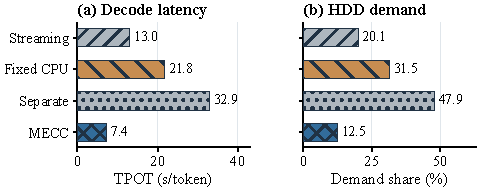
\includegraphics[width=\columnwidth]{measured_figures/intro_evidence.pdf}
\par\nointerlineskip
\caption{Local retention controls on one A100 with Mixtral-8x7B. Separate denotes independently managed HBM/CPU caches. All policies use the same nominal slots and eight-prompt input. HDD-demand share includes all instrumented phases. One run per policy.}
\label{fig:intro}
\end{figure}

We present \mecc{}, the MoE Expert Cache Compiler, to connect initial placement with runtime retention. An independent route profile supplies an expert-demand prior. The compiler ranks experts within each layer and allocates HBM and CPU slots under the task's allowances. Each plan retains the profiled layer/expert IDs, since equal indices in different layers refer to different weights. At runtime, the unchanged router provides actual demand. A CPU hit promotes the selected expert and retains the displaced HBM expert in CPU memory, preserving it for later tokens. Online recency changes the resident identities as the workload changes, while the compiled capacities remain fixed. Weight delivery orders reads, copies, and GPU consumers through readiness dependencies. These decisions address different parts of the same lifecycle: the profile selects an initial state, joint retention preserves reuse, and the delivery contract makes requested weights available before execution. The current A100 evaluation uses uniform initialization to examine runtime behavior independently of a profile-placement gain.

This paper makes three contributions.
\begin{list}{}{\setlength{\leftmargin}{16pt}\setlength{\labelwidth}{14pt}\setlength{\labelsep}{2pt}\setlength{\itemsep}{3pt}\setlength{\topsep}{3pt}}
\item[(1)] \textbf{Placement compilation:} we define a per-layer interface that maps route profiles and task allowances to ranked expert IDs and initial tier capacities, together with a marginal-coverage allocation heuristic.
\item[(2)] \textbf{Joint retention and delivery:} we specify promotion, victim demotion, and readiness dependencies across HBM, CPU pinned memory, and HDD while retaining the router and FP16 weights.
\item[(3)] \textbf{Single-GPU evaluation:} we implement an end-to-end harness and compare the runtime with streaming, fixed-CPU retention, independent caches, and local alternative policies on Mixtral-8x7B. With uniform initialization, MECC takes 7.38~s per output token, compared with 13.04~s for streaming and 21.75~s for fixed-CPU retention; the latter two controls report the same sample perplexity as MECC. The evaluation also examines source-tier demand and host-slot sensitivity.
\end{list}
\twocolumn[{
\begin{minipage}{\textwidth}
\centering
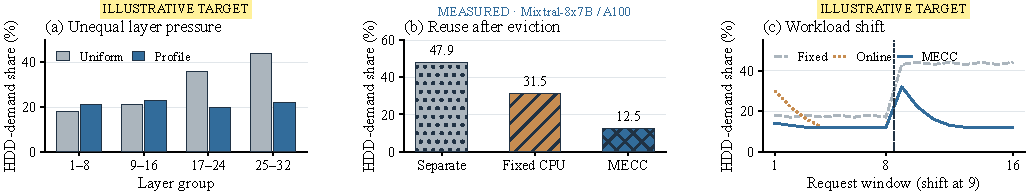
\includegraphics[width=\textwidth]{completion_figures/motivation_evidence.pdf}\par
\vspace{2pt}
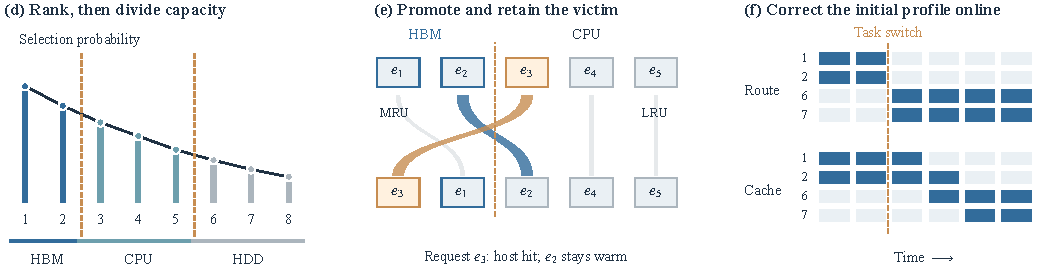
\includegraphics[width=\textwidth]{measured_figures/insights_lower.pdf}
\par\nointerlineskip
\captionof{figure}{Motivation evidence and matching insights. \pending{Panels (a,c) are ideal targets to replace}; (b) is measured A100 demand across all phases. (d--f) are schematic mechanisms, adapted from the talk. Profiles guide initial coverage, joint retention preserves victims, and online updates follow changed routing.}
\label{fig:insights}
\vspace{5pt}
\end{minipage}
}]
\section{Background}
\label{sec:background}
An MoE layer routes each token to a small subset of its experts. Sparse execution reduces arithmetic, but every expert remains a possible future selection~\cite{shazeer,switch,gshard}. Mixtral and the DeepSeek family instantiate this separation between active computation and total weights~\cite{mixtral,deepseekmoe,deepseekv2,deepseekv3,mixtral22}. Experts with the same index in different layers are different weight objects. A route profile must therefore retain both layer and expert identity.

Expert parallelism partitions weights over resident GPU memories and dispatches token activations to their owners~\cite{deepspeedmoe,tutel,megablocks,flashmoedist,harmoeny}. On one GPU, the task also needs space for dense layers, activations, and the KV cache. KV management and request execution are complementary to expert residency~\cite{pagedattention,sglang}. A host-resident expert needs an H2D copy; an expert absent from both fast tiers additionally needs a backing-store read. Heterogeneous inference systems expose related placement and scheduling choices~\cite{flexgen,dsinference,zeroinfinity,llmflash,powerinfer}.

We use immutable FP16 experts and three logical tiers: HBM, CPU pinned memory, and HDD. The task's allowance may be smaller than the server's physical RAM. Unique resident weights, host mirrors, staging buffers, and other allocations must be distinguished. The original gate determines demand, and a delivered expert can remain resident for later tokens. MECC separates the initial residency decision from the online transitions that respond to those later selections.

\section{Motivation and Insights}
\label{sec:challenges}
\subsection{Spend Capacity Where It Covers Demand}
Equal slots per layer assume comparable cache pressure. A profile can reveal different ranked demand distributions even when each layer has the same expert count. Figure~\ref{fig:insights}(a,d) connects this question to a ranked capacity cut: the compiler allocates the next slot by its marginal covered demand. \pending{E05: replace panel (a)'s ideal numbers with a same-runtime, same-byte placement sweep.} The experiment must include empirical-profile and uniform controls; the current measured main runs use uniform initialization. Local routing consistency can also vary across models~\cite{routingconsistency}.

\subsection{An HBM Victim Can Still Be Useful}
Figure~\ref{fig:insights}(b,e) shows why two resident sets should preserve cross-tier reuse. With the same nominal slots and initialization, the measured independent-cache control reports 47.9\% HDD demand, fixed CPU 31.5\%, and MECC 12.5\%. These counters span all instrumented phases. The insight is to promote a host hit while retaining the displaced HBM expert in CPU, rather than treating the eviction as the end of its useful lifetime. The source-tier and physical-byte measurements answer different questions and must be reported separately.

\subsection{Use the Profile as an Initial State}
A profile represents past inputs. If the routed set changes, fixed residency can preserve experts that are no longer useful. Figure~\ref{fig:insights}(c,f) pairs an expected miss transient with the corresponding residency update. Compilation fixes capacities and ranked IDs; online recency changes identities within those capacities. \pending{E07/E08: measure initial misses and the WikiText-2/GSM8K switch transient using distinct, hashed input sets.} The experiment must retain the no-switch control and compare profile-plus-online with both fixed residency and online-only initialization.

\twocolumn[{
\begin{minipage}{\textwidth}
\section{Overview}
\label{sec:overview}
\centering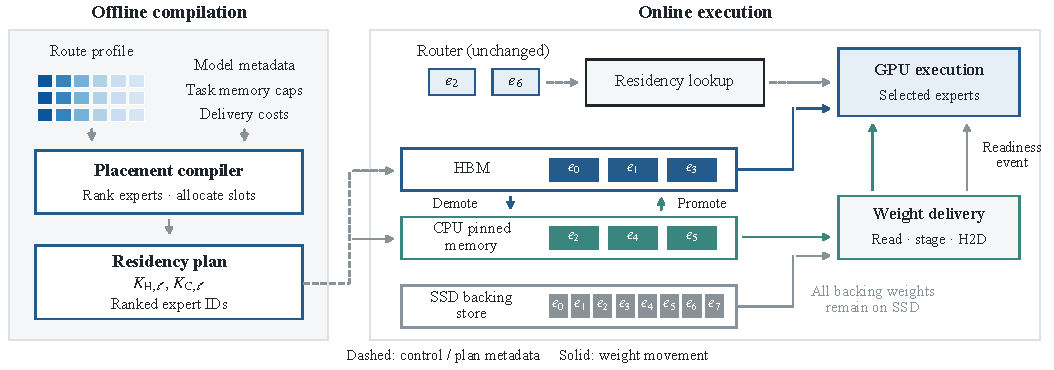
\includegraphics[width=\textwidth]{figures/fig01_overview.pdf}
\par\nointerlineskip
\captionof{figure}{MECC framework. The placement compiler emits per-layer capacities and ranked IDs. Online execution resolves unchanged router selections against HBM, CPU pinned memory, and HDD, then delivers weights before their GPU consumers. Dashed arrows carry control or plan metadata; solid arrows move weights.}
\label{fig:overview}

\vspace{8pt}
\end{minipage}
}]



Figure~\ref{fig:overview} separates offline compilation from online execution. An independent route profile, model metadata, task memory caps, and delivery costs define the compilation inputs. The output specifies layer capacities and initial expert IDs. Mirrors and staging are charged outside unique primary residency; HDD retains all backing weights.

The unchanged router supplies demand IDs. Residency lookup selects a source tier; the runtime promotes requested experts and demotes HBM victims. The delivery path enforces weight readiness before execution. Layer capacities stay fixed during a run, while expert identities and recency change. Planner controls therefore fix online rules; replacement controls fix quotas and initialization (Section~\ref{sec:mechanisms}).

\section{Method}
\label{sec:method}
\subsection{Compiler: Profile-Guided Placement}
\begin{figure}[H]
\centering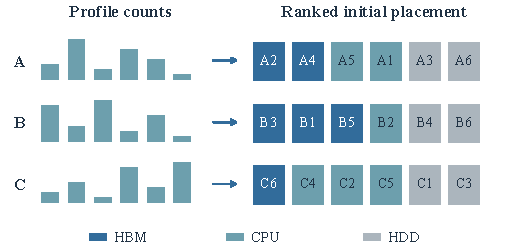
\includegraphics[width=\columnwidth]{measured_figures/method_compile.pdf}
\par\nointerlineskip
\caption{Compiling layer-specific placement. A, B, and C denote different layers. The compiler keeps each layer's expert identities, ranks its profile counts, and allocates HBM and CPU slots from shared task allowances. Colors identify initial tiers; counts and capacities are schematic.}
\label{fig:compile}
\end{figure}
Figure~\ref{fig:compile} shows the compiler's input and emitted state.
The compiler takes model metadata, memory budgets, delivery costs, and an independent route profile. The profile supplies request probability $p_e$ for each expert. For equal-size experts within a layer, a discrete Zipf model summarizes the ranked probabilities:
\begin{equation}
 q_{\ell,r}=\frac{r^{-\alpha_\ell}}{H_{N_\ell}(\alpha_\ell)},\qquad
 H_n(\alpha)=\sum_{r=1}^{n}r^{-\alpha}.
\end{equation}
Here $q_{\ell,r}$ is conditional on an expert selection in layer $\ell$. Let $w_\ell$ be that layer's fraction of all selections. The global probability is $p_e=w_\ell q_{\ell,r}$, with $\sum_\ell w_\ell=1$. For fixed top-$k$ routing, $w_\ell=k_\ell/\sum_j k_j$. Each rank retains its profiled expert ID. Empirical probabilities can replace the fitted Zipf distribution. Neither representation encodes request order.

Let $x_{e,t}\in\{0,1\}$ indicate the primary tier of expert $e$. The tiers are HBM, CPU, and HDD, denoted by $\mathrm H$, $\mathrm C$, and $\mathrm S$. Residency budgets $\bar B_t$ must exclude buffers and mirrors. The following static objective is a reference model, not a claim that the current planner solves the full problem:
\begin{align}
 \min_x\quad &\sum_e p_e\sum_t x_{e,t}T_t(s_e),\label{eq:placement}\\
 \text{s.t.}\quad&\sum_t x_{e,t}=1,\quad
 \sum_e s_e x_{e,t}\le \bar B_t\quad(t\in\{\mathrm H,\mathrm C\}).\nonumber
\end{align}
The affine model $T_t(s)=a_t+s/b_t$ represents fixed overhead and effective bandwidth. Calibration uses the target machine. Equation~\ref{eq:placement} estimates static delivery cost under the profile. Runtime locality, migration, and overlap are evaluated separately.

For equal-size experts with fixed probabilities, exchanging a more probable expert in a slower tier with a less probable expert in a faster tier cannot increase static expected cost. This establishes ranked placement under independent capacities and ordered tier costs. The implementation below uses marginal coverage, rather than claiming to solve the general latency objective.

The multilayer implementation allocates slots by marginal coverage. Under the Zipf model, a slot covering rank $r$ adds
\begin{equation}
 \Delta_{\ell}(r)=w_\ell q_{\ell,r}.
\end{equation}
This is a coverage score, not the exact latency marginal of Equation~\ref{eq:placement}. Tier-boundary movements can affect both HBM and CPU assignments. The heuristic allocates HBM slots first, then CPU slots from the remaining ranks. At each step it selects the largest next-rank score; ties use layer ID. Expert-ranking ties use expert ID. It stops at the tier's slot cap or exhaustion of experts. Per-layer minima, if enabled, are assigned first and an infeasible minimum allocation must be rejected. A direct scan costs $O(L(S_{\mathrm H}+S_{\mathrm C}))$ after ranking, where $S_t$ is a total slot cap. These rules define the compiler interface. Batched prefill additionally requires distinguishing token selections from distinct expert fetches. The sequential heuristic does not solve the general static objective.

The plan records per-layer capacities, ranked expert IDs, initial tiers, and modeled hit fractions. A missing profile selects natural expert order. The measured runs below use this uniform/natural-order path, so they test the runtime retention and delivery stack rather than the profile compiler. Profile initialization cost and gains require separate matched runs.

\subsection{Runtime: Cross-Tier Retention}
Each layer has ordered HBM and CPU residency maps. An HBM hit updates recency. A CPU hit removes the expert from CPU residency and promotes it to HBM as most recently used. An HDD miss reads the weights into staging before H2D transfer. When HBM is full, its least-recently used expert is demoted to CPU. CPU pressure evicts the least-recently used host resident. The HDD backing weights remain available.

Figure~\ref{fig:retention} starts with HBM $[e_1,e_2]$ and CPU $[e_3,e_4]$, each ordered from MRU to LRU. Requesting $e_3$ promotes it and demotes $e_2$. A later request for $e_2$ hits CPU. This example uses exclusive logical residency. An implementation can keep a CPU mirror to avoid device-to-host (D2H) transfer on eviction. The mirror consumes host memory and is charged separately.

\begin{figure}[H]
\centering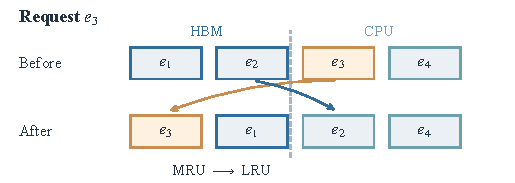
\includegraphics[width=\columnwidth]{measured_figures/method_runtime.pdf}
\par\nointerlineskip
\caption{One CPU-hit transition. Lists run from MRU to LRU. Requesting $e_3$ promotes it, demotes the HBM victim $e_2$, and preserves both experts in the combined fast-tier set. The dashed line is the capacity boundary.}
\label{fig:retention}
\end{figure}

For a serial demand stream within one layer, concatenate the HBM MRU-to-LRU stack with the CPU MRU-to-LRU stack. Exclusive promotion and victim demotion preserve the corresponding LRU stack of capacity $\KH+\KC$. This reference requires matching initialization, no prefetch or alternative admission, and completed transitions before the next request. It does not imply equivalence to a cache that reallocates capacity across layers, or dominance over static placement.

\subsection{Delivery: Dependency-Aware Overlap}
A correct asynchronous implementation requires a readiness event after each pinned-host copy. The computation stream must wait before consuming the weight. The source buffer must remain live until copy completion, and the resident weight until its last consumer finishes. These are required lifetime rules, including across separate loading and dispatch iterators; the execution stream must enforce them with readiness events.

At batch one, routing reveals the selected IDs only after the current layer's gate. Copying one selected expert may overlap computation of another already-ready expert if kernel and aggregation order permit. This provides no knowledge of a later layer's route. In-flight weights must be protected from eviction. Replacement comparisons must disable predictive prefetch; the overlap control must hold admission, residency, and requests fixed. The available overlap and its exposed critical path remain measurements, rather than an assumed gain from a copy stream.

Figure~\ref{fig:delivery} pairs HBM-resident $e_1$ with HDD-backed $e_3$ from the same gate. HDD read precedes H2D and readiness. Copy completion releases the pinned source; final-consumer completion permits GPU eviction. Useful independent computation determines the available overlap.

\begin{figure}[H]
\centering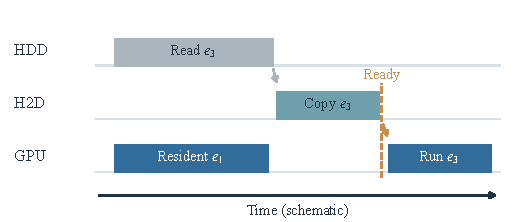
\includegraphics[width=\columnwidth]{measured_figures/method_delivery.pdf}
\par\nointerlineskip
\caption{Delivery dependencies within one gate's selected set. The GPU can execute resident $e_1$ while $e_3$ is read and copied. A readiness event orders the copied weight before its GPU consumer. Durations are schematic.}
\label{fig:delivery}
\end{figure}

The design requires unchanged weights, selected experts, kernels, and aggregation order. Under these conditions, changing residency preserves the forward computation. The implementation also needs correct synchronization. The validation protocol compares synchronous and asynchronous paths on identical inputs using weight hashes, route selections, logits, tokens, and perplexity; the same protocol isolates transfer scheduling from changes in numerical execution.

\subsection{Implementation and Accounting}
Policies share the FP16 loader and unchanged router. Logical tier occupancy is not physical memory. Host mirrors, staging, and temporary copies are charged separately from unique residents. Full CPU mirroring requires host bytes at least as large as the mirrored HBM experts. \pending{E14: replace nominal slot equivalence with measured physical-byte accounting.}

The harness records initialization, warmup, prefill, decode, and PPL separately. TPOT and TTFT use their own timing windows. Demand-source counts and physical HDD/H2D/D2H bytes must share phase boundaries. \pending{E15: complete independent-resident reference checks before a general lossless claim.}

\section{Evaluation}
\label{sec:evaluation}
\subsection{Testbed and Evidence Map}
Measured runs use FP16 Mixtral-8x7B-Instruct-v0.1 on one A100 80~GB PCIe. The cold store is on a RAID logical device reporting rotational media; physical drives remain uninventoried. Main runs use four HBM and three host slots per layer, uniform initialization, eight WikiText-2 prompts, 64 input and 64 output tokens, and one run per policy. Perplexity uses 1024 WikiText-2 tokens. The 50/40~GB allowances are planner parameters; mirrors and buffers still need a physical-byte audit.

Yellow plots and text are experiment-completion targets, not measurements. Their arrays come from the existing design-target record. \pending{Freeze model revisions, input hashes, precision, total charged bytes, and timing windows before replacing each target.} The experiments address full-system benefit, individual mechanisms, workload change, resource tradeoffs, and numerical equivalence.

\begin{figure*}[!t]
\centering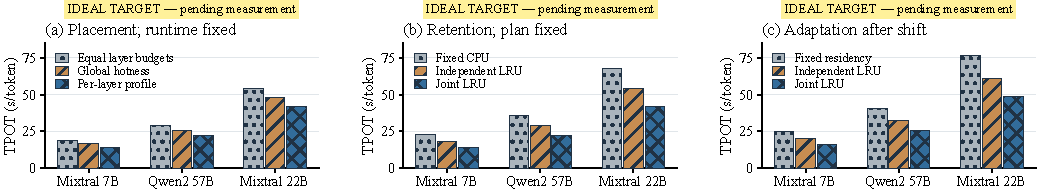
\includegraphics[width=\textwidth]{completion_figures/mechanism_sweeps.pdf}
\par\nointerlineskip
\caption{\pending{TO MEASURE: ideal component targets on three models.} (a) Placement with runtime fixed. (b) Retention with initialization fixed. (c) Adaptation after a task switch. Separate protocols must be frozen for the three controls; these bars are not A100 outcomes.}
\label{fig:target_mechanisms}
\end{figure*}

\subsection{Measured Runtime and Quality}
\begin{figure}[H]
\centering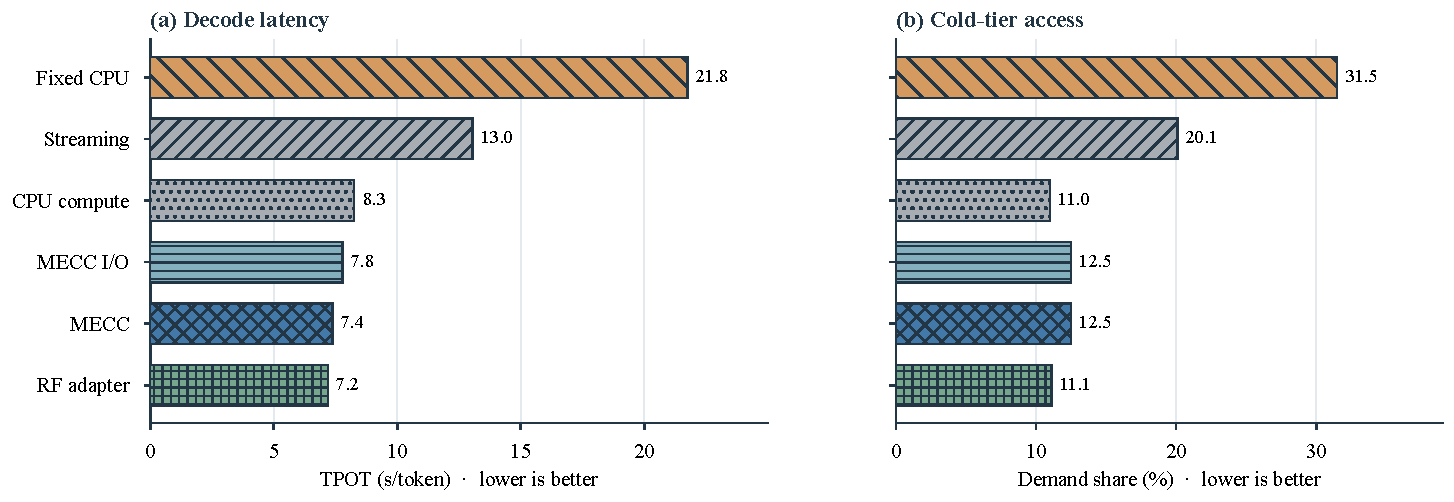
\includegraphics[width=\columnwidth]{measured_figures/main.pdf}
\par\nointerlineskip
\caption{Measured single-A100 runtime: one run per local policy, eight WikiText-2 prompts, 64 output tokens. RF and CPU-compute adapters are local mechanisms.}
\label{fig:performance}
\end{figure}
Figure~\ref{fig:performance} reports MECC at 7.38~s/token, streaming at 13.04, and fixed CPU at 21.75: TPOT ratios of 1.77$\times$ and 2.95$\times$. The RF adapter takes 7.19~s, MECC I/O 7.78, and CPU compute 8.26. RF is faster than MECC in this run. MECC's TTFT is 139.1~s, versus 156.9 for streaming and 174.2 for fixed CPU. MECC, streaming, fixed CPU, RF, and MECC I/O report PPL 3.427; CPU compute reports 3.432. A short-window route/logit/token diagnostic supports local correctness but does not replace an independent resident reference.

\subsection{Mechanism Attribution}
\label{sec:mechanisms}

The matched local independent-cache control takes 32.94~s/token. Figure~\ref{fig:target_mechanisms} separates three mechanisms in the target component harness. For Mixtral-8x7B, the placement target moves from \pending{18.6 to 14.2 s/token}, joint retention from \pending{18.3 to 14.2}, and post-switch adaptation from \pending{25.1 to 16.0} relative to fixed residency. The three controls hold runtime, initial plan, and switch protocol fixed, respectively. This separates better initial coverage from preservation of later reuse. \pending{E04--E08: replace targets and add leave-one-out controls.}

\begin{figure}[H]
\centering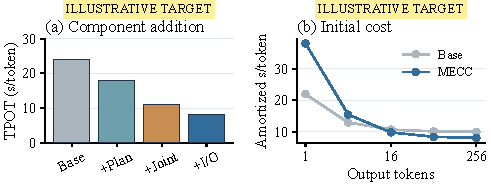
\includegraphics[width=\columnwidth]{completion_figures/ablation_startup.pdf}
\par\nointerlineskip
\caption{\pending{TO MEASURE: ideal ablation and startup targets.} The right panel evaluates startup/output-token plus decode cost from authored inputs; it is not a measured latency trace.}
\label{fig:target_ablation}
\end{figure}
Figure~\ref{fig:target_ablation} tests component addition and startup amortization. The authored TPOT sequence is \pending{24, 18, 11, and 8 s/token}. The last I/O step retains a \pending{20-percent target HDD-demand share}, separating delivery scheduling from miss reduction. With the plotted startup/decode costs, the target amortization curves cross at \pending{9 output tokens}. This check exposes the service horizon over which an initial investment pays back. \pending{E04/E13: replace targets with phase timings and addition/removal runs.}

\subsection{Model and Deployment Coverage}
\begin{figure}[H]
\centering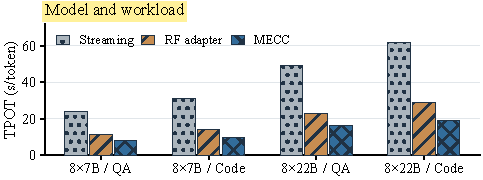
\includegraphics[width=\columnwidth]{completion_figures/cross_model.pdf}
\par\nointerlineskip
\caption{\pending{TO MEASURE: ideal model/workload targets.} Mixtral-8x7B and 8x22B with QA/code inputs. Values specify planned comparisons, not measured benchmarks. The RF policy is a local adapter.}
\label{fig:target_models}
\end{figure}
Figure~\ref{fig:target_models} expands the present one-model workload. The MECC target ranges from \pending{8 to 19 s/token}, versus \pending{24 to 62} for streaming and \pending{11 to 29} for the RF adapter. QA and code exercise different expert-demand patterns; increasing model size also changes the expert pool and transfer size. The comparison therefore pairs every policy within each model/workload point. \pending{E01/E02: replace targets under frozen inputs, precision, and byte allowances.}

\begin{figure}[H]
\centering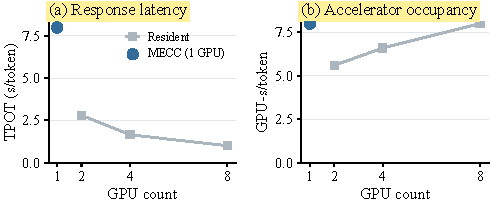
\includegraphics[width=\columnwidth]{completion_figures/gpu_tradeoff.pdf}
\par\nointerlineskip
\caption{\pending{TO MEASURE: ideal one-GPU/resident-reference tradeoff.} MECC has only a one-GPU point. Resident points use 2/4/8 GPUs; occupancy is GPU count times TPOT. These values are not published FlashMoE results.}
\label{fig:target_gpu}
\end{figure}
Figure~\ref{fig:target_gpu} separates GPU provisioning from response latency. The endpoint target is \pending{one GPU at 8 s/token versus eight GPUs at 1 s/token}; both correspond to \pending{8 GPU-s/token}. The \pending{two-GPU resident target is 5.6 GPU-s/token}, which makes the smallest feasible resident configuration a necessary comparison. Occupancy is reported alongside latency, rather than substituted for energy. \pending{E03/E14: replace all resident-reference targets.}

\balance
\subsection{Capacity and Implementation Checks}
\begin{figure}[H]
\centering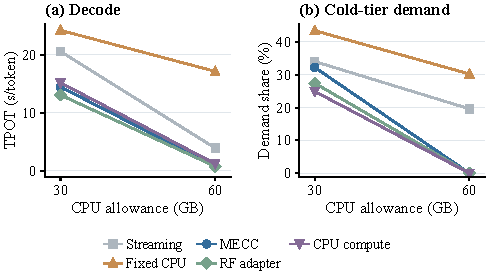
\includegraphics[width=\columnwidth]{measured_figures/budget.pdf}
\par\nointerlineskip
\caption{Measured 30/60~GB nominal host-allowance comparison. Four WikiText-2 prompts and 16 output tokens, one run per point. Demand share covers all instrumented phases.}
\label{fig:budget}
\end{figure}
Figure~\ref{fig:budget} reports MECC at 14.46 and 0.76~s/token, with 32.2\% and zero HDD demand. Four HBM plus four host slots at 60~GB cover all eight experts per layer; zero cold demand is a capacity transition. RF takes 13.06 and 0.74~s/token. These points use a shorter protocol than the main run.

\begin{figure}[H]
\centering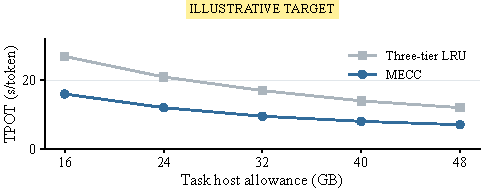
\includegraphics[width=\columnwidth]{completion_figures/quota_targets.pdf}
\par\nointerlineskip
\caption{\pending{TO MEASURE: ideal dense-quota sweep.} The target experiment uses a separately frozen protocol; it is not joined to the measured 30/60~GB curve.}
\label{fig:target_quota}
\end{figure}
Figure~\ref{fig:target_quota} resolves intermediate capacity points. Its authored MECC target changes from \pending{16 to 7 s/token} over \pending{16--48 GB}, compared with \pending{27 to 12} for three-tier LRU. The purpose is to separate pressure within the cold-tier regime from the full-coverage threshold. \pending{E10: replace with one matched, physically charged quota sweep.}

\pending{E14/E15: fill peak physical HBM/host bytes, mirrors, pinned staging, phase-specific traffic, and independent-reference route/logit/token checks.} The current sample PPL equality supports only that sample. \pending{E09/E11/E12: add profile-size sensitivity, no-switch/shift controls, and batch/input/output-length sensitivity if the corresponding claims remain in the paper.}

\begin{table}[H]
\centering\small\renewcommand{\arraystretch}{0.9}
\caption{Numerical and resource checks. Sample PPL values are measured; highlighted entries require independent validation or measurement.}
\label{tab:checks}
\begin{tabular}{@{}p{0.46\linewidth}p{0.49\linewidth}@{}}
\toprule
Check & Current value / target\\
\midrule
MECC / fixed-CPU sample PPL & 3.427 / 3.427\\
CPU-compute sample PPL & 3.432\\
Resident-reference route match & \pending{Target: exact}\\
Resident-reference logit error & \pending{Target: zero}\\
Physical HBM / host peak bytes & \pending{TO MEASURE}\\
Phase-specific HDD/H2D bytes & \pending{TO MEASURE}\\
\bottomrule
\end{tabular}
\end{table}
Table~\ref{tab:checks} closes the evaluation contract: performance comparisons preserve the routed computation and precision, and charge the actual resident and temporary allocations. A nominal slot budget alone cannot establish physical-memory equivalence.

\section{Related Work}
Expert offloading starts from the distinction between sparse execution and full weight capacity~\cite{offloading,swapmoe}. Fiddler and DAOP choose CPU/GPU execution or movement; MoE-Lightning pipelines heterogeneous work; MoE-Infinity uses activation traces~\cite{fiddler,daop,lightning,moeinfinity}. ProMoE, Pre-gated MoE, Fate, and ExpertFlow provide lookahead, proactive caching, or token scheduling~\cite{promoe,pregated,fate,expertflow}. MECC's demand path instead consumes the original gate output and coordinates initial placement with online residency.

HOBBIT and Specter use precision in expert loading; MoEpic divides experts into segments; SliceMoE caches precision slices; Mira combines staging with quantization~\cite{hobbit,specter,moepic,slicemoe,mira}. ZipMoE uses compression and affinity scheduling~\cite{zipmoe}. SSD-LLaMA, edge FlashMoE, and MoE-CORE address storage delivery, replacement, or coordinated residency~\cite{ssdllama,flashmoe,core}. MECC studies the interaction between an independent placement prior and online whole-expert retention across the two fast tiers under HDD-backed demand.

Granularity changes the meaning of a cache hit. A segment cache can avoid part of an expert transfer while still fetching the remaining weights. A precision-slice cache can change both resident bytes and numerical execution. A whole-expert cache instead changes the source of unchanged weights. These comparisons therefore report representation and quality alongside latency. Physical traffic per miss and the number of misses are separate quantities: compression or splitting can reduce the former, while retention changes the latter.

\begin{table}[H]
\centering\small\renewcommand{\arraystretch}{0.9}
\caption{Representative control granularity and primary decision.}
\label{tab:related_units}
\begin{tabular}{@{}p{0.20\linewidth}p{0.22\linewidth}p{0.47\linewidth}@{}}
\toprule
System & Unit & Primary decision\\
\midrule
Fiddler~\cite{fiddler} & Expert & CPU/GPU execution\\
ProMoE~\cite{promoe} & Expert & Proactive caching\\
MoEpic~\cite{moepic} & Segment & Split ratio and allocation\\
HOBBIT~\cite{hobbit} & Expert precision & Precision-aware loading\\
Bevy~\cite{bevy} & Request & Runahead and batching\\
MECC & FP16 expert & Initial placement and joint retention\\
\bottomrule
\end{tabular}
\end{table}

Klotski and Bevy expose independent work across batches or requests~\cite{klotski,bevy}. OD-MoE distributes on-demand loading over edge nodes, while HeteGen studies heterogeneous dense-model inference~\cite{odmoe,hetegen}. Their execution units differ from batch-one per-gate expert delivery. The full-system, mechanism, and resource experiments above distinguish these comparisons.

Cross-request scheduling also changes the available overlap. A ready request can advance while another waits, providing work beyond the current gate's selected experts. In a single-request stream, MECC's delivery dependencies only expose already-ready expert computation. This distinction explains why cache replacement, route lookahead, and request scheduling require separate controls even when all three improve an end-to-end latency metric.

\section{Conclusion}
MECC connects a profile-derived initial state with online cross-tier retention and weight delivery. Current single-A100 measurements support the local runtime comparison. The yellow experiment panels define the remaining evidence for placement, adaptation, model coverage, startup, and resident multi-GPU tradeoffs. They must be replaced before those outcomes enter a final performance claim.

\clearpage
\nobalance
\IEEEtriggeratref{24}
\bibliographystyle{IEEEtran}
\bibliography{references}
\end{document}
